\documentclass[czech,bachelor]{diploma}

\usepackage[autostyle=true,czech=quotes]{csquotes}
\usepackage[backend=biber, style=iso-numeric, alldates=iso]{biblatex}
\usepackage{dcolumn}
\usepackage{subfig}
\usepackage[cpp]{diplomalst}

\addbibresource{biblatex.bib}

\ThesisAuthor{Ratmir Gaitov}
\ThesisSupervisor{Ing. Petr Olivka, Ph.D.}
\CzechThesisTitle{Autonomní řízení auto - optimalizace řízení dle pohybových senzorů}
\EnglishThesisTitle{Autonomous Car Control - Speed Optimization According to Motion Sensors}
\SubmissionYear{2024}
\ThesisAssignmentFileName{ThesisAssignment.pdf}

\Acknowledgement{Rád bych na tomto místě poděkoval mého vědoucího Petra Olivku, který mi s prací pomohl, protože bez nich by tato práce nevznikla.}

\CzechAbstract{
Tato práce popisuje ovládání modelu automobilu používaného na mezinárodní soutěží NXP Cup, konkretně korigování rychlosti jízdy pomocí pohybových senzorů.
Jsou provedeny testy různých senzoru a signálových filtru, ze kterých pak vybraná nejlepší konfigurace.
Tyto vybrané signálové filtry pak implementovaný v kombinace se vhodnými senzory.
}
\CzechKeywords{Automatické regulování rychlosti; Signálové filtry; NXP Cup; FRDM-K66F}

\EnglishAbstract{This paper describes the control of a model car used in the international NXP Cup competition, specifically the correction of driving speed using motion sensors.
Tests of different sensor and signal filters are performed, from which the best configuration is then selected.
These selected signal filters are then implemented in combination with suitable sensors.}
\EnglishKeywords{Automatic speed control; Signal filters; NXP Cup; FRDM-K66F}

\AddAcronym{MCU}{Micro Controller Unit}
\AddAcronym{PWM}{Pulse Width Modulation}
\AddAcronym{GPIO}{General-Purpose Input/Output}
\AddAcronym{NiMH}{Nickel-Metal Hydride}
\AddAcronym{WiFi}{Wireless Fidelity}
\AddAcronym{ARM}{Advanced RISC Machine}
\AddAcronym{RAM}{Random Access Memory}
\AddAcronym{LED}{Light-Emitting Diode}
\AddAcronym{SDHC}{Secure Digital High Capacity}
\AddAcronym{MEMS}{Micro-Electro-Mechanical System}
\AddAcronym{IMU}{Inertial Measurement Unit}

\newcolumntype{d}[1]{D{,}{,}{#1}}

\begin{document}
\MakeTitlePages

\listoffigures
\clearpage

\listoftables
\clearpage

\chapter*{Úvod}
\label{sec:Introduction}
\addcontentsline{toc}{chapter}{\protect\numberline{}Úvod}\

Autonomní řízení automobilů je v~současné době velmi populárním tématem, přičemž
výrobci automobilů se předhánějí o~prvenství v~této oblasti. Jedná se především
o~velmi komplexní oblast, kde musí být správně vyřešeny všechny možné situace, jelikož
jakýkoliv přehlédnutý detail může způsobit újmu na zdraví. Z~tohoto důvodu je
autonomní řízení částí populace stále vnímáno jako něco  nepřijatelného, ovšem
zvyšující se rychlost vývoje naznačuje, že v~následujících letech dojde k~významnému
pokroku v~této oblasti a~setkávání autonomně řízenými auty bude běžným jevem.

V~této bakalářské práci bude popsán způsob automatického řízení auta a~korekce 
rychlosti na základě informací z~pohybových senzorů. Práce začne popisem modelu 
automobilu pro testování. Následně budou popsány algoritmy pro automatické a~manuální 
řízení. Další část se bude zabývat metodami pro zobrazování a~ukládání hodnot dat auta 
během jízdy. Poté budou otestovány a~vybrány vhodné senzory a~filtry pro detekci fáze 
jízdy. V~závěrečné části práce bude popsán algoritmus pro optimalizaci rychlosti 
a~provedeno porovnání s~manuálním řízením.

\endinput
\chapter{Model automobilu}
\label{sec:CarModel}\

V~této kapitole je popsán model automobilu a~jeho jednotlivé součásti.

Model automobilu je založen na podvozku typu Alamak, která má \textbf{1 servomotor}
pro řízení a~\textbf{2 motory} pro pohon. \textbf{Podvozek Alamak} je řízen pomocí 
\textbf{NXP Freedom K66F} spolu s~modulem \textbf{POLI-TFC} 
přípojeným do GPIO pinů MCU. Detailní popis MCU a~modulu jsou v~podkapitolách 
\ref{sec:FRDM-K66F} a~\ref{sec:POLI-TFC}.

Pro manuální řízení je zapojen přijímač RC signálu \textbf{Minima 6S} do pinu
POLI-TFC shieldu. Přijímač pak přijímá signály z~vysílače \textbf{Hitec OPTIC 6 
SPORT}.

Pro komunikaci s~podvozkem Alamak je použit \textbf{WiFi Access Point}, který je
připojen k~MCU pomocí Ethernet portu. \textbf{Řádková kamera}, která je umístěna
v~přední části, se používá pro získání obrazu dráhy. Všechny součástky
jsou napájeny baterií typu \textbf{NiMH} o~napětí 7,2 V.

Celý model je zobrazen na obrázku \ref{fig:car}.
\begin{figure}[!h]
    \centering
    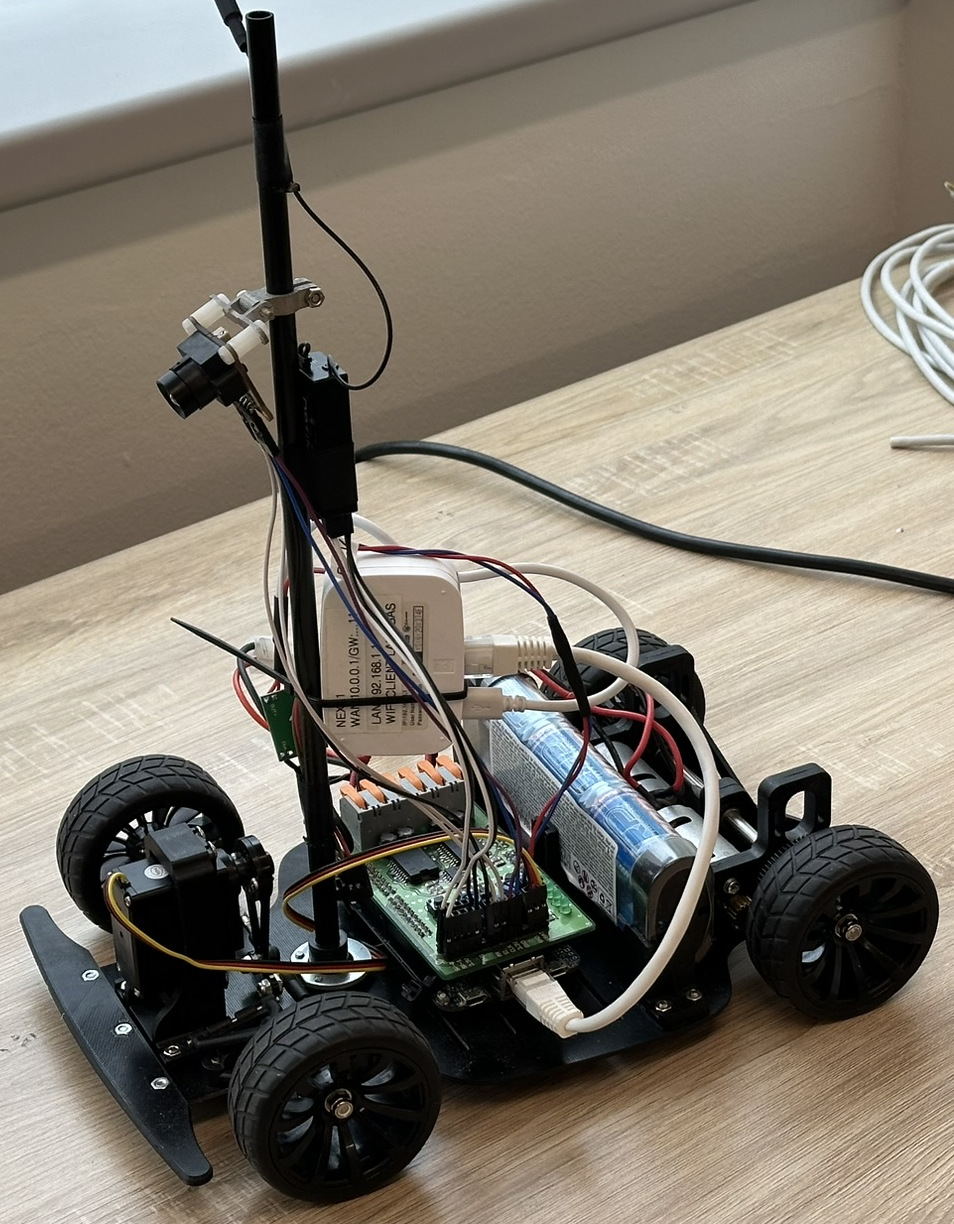
\includegraphics[width = .4\linewidth]{Figures/Car.jpeg}
    \caption{Model auta.}
    \label{fig:car}
\end{figure}

\section{FRDM-K66F}
\label{sec:FRDM-K66F}\

\textbf{FRDM-K66F} je vývojová platforma od společnosti NXP určená pro MCU řady 
Kinetis K66 a~K26. Platforma je založena na jádře \textbf{ARM© Cortex®-M4}
a~využívá model \textbf{MK66FN2M0VMD18} s~frekvencí 180 MHz, 2 MB flash paměti
a~256 KB RAM \cite{frdmk66UserGuide}.

Konektivitu zajišťují 2 micro-B USB porty, 1 ethernetový port a~54 GPIO pinů.
GPIO~piny jsou kompatibilní s~\textbf{Arduino™ R3}, čímž je poskytnuta široká škála
možností pro rozšiřující desky. Deska umožňuje bezdrátové možností konektivity
pomocí modulů Bluetooth a~RF \cite{frdmk66UserGuide}.

Pro ladění je na platformě přítomno rozhraní \textbf{OpenSDAv2.1}, které podporuje
J-Link. J-Link~je sériový programovací adaptér, který umožňuje programování
a~debugování mikrokontrolérů \cite{frdmk66UserGuide}.

Další užitečné periferie na desce zahrnují trojbarevnou LED, SDHC a~digitální MEMS
mikrofon~\cite{frdmk66UserGuide}.

Jako \textbf{inerciální měřicí jednotku} (IMU) platforma využívá akcelerometr
společně s~magnetometrem a~gyroskopem \cite{frdmk66UserGuide}.

Vývojová platforma je znázorněna na obrázku \ref{fig:FRDM-K66F}.

\section{POLI-TFC}
\label{sec:POLI-TFC}\

\textbf{POLI-TFC shield} je rozšiřující deska pro FRDM-K66F, která rozšiřuje
rozhraní pro připojení periferií k~vývojové desce. Shield obsahuje 2 konektory
pro motory, 2 servomotory, 2 rozhraní pro~připojení řádkových kamer, 2 
potenciometry, 4 DIP přepínače a~4 LED diody. 

Shield~je zobrazen na obrázku \ref{fig:POLI-TFC}.

\begin{figure}[h]
    \begin{subfigure}{0.45\textwidth}
        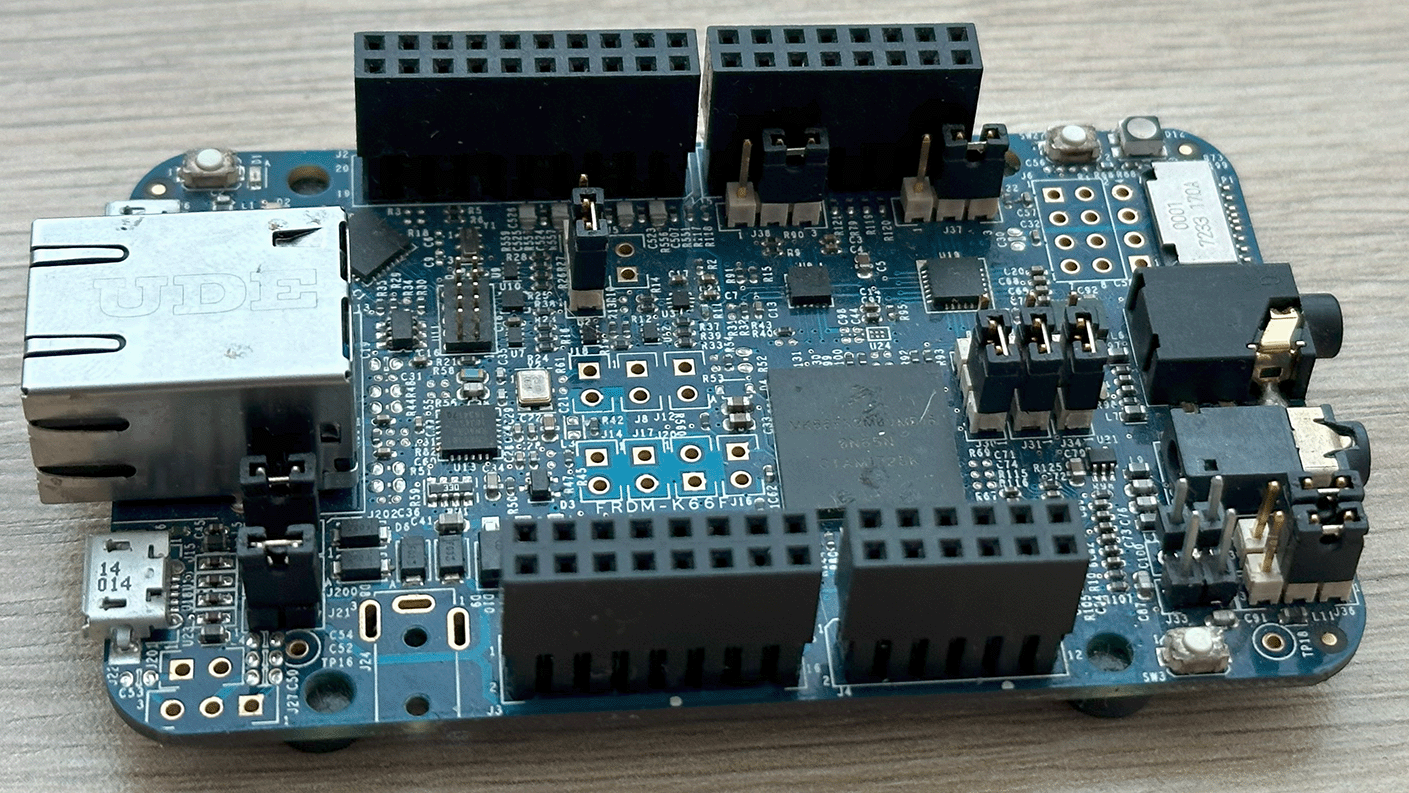
\includegraphics[width=\textwidth, height = 5cm]{Figures/FRDM-K66F.png} 
        \caption{FRDM-K66F.}
        \label{fig:FRDM-K66F}
    \end{subfigure}
    \hfill
    \begin{subfigure}{0.45\textwidth}
    	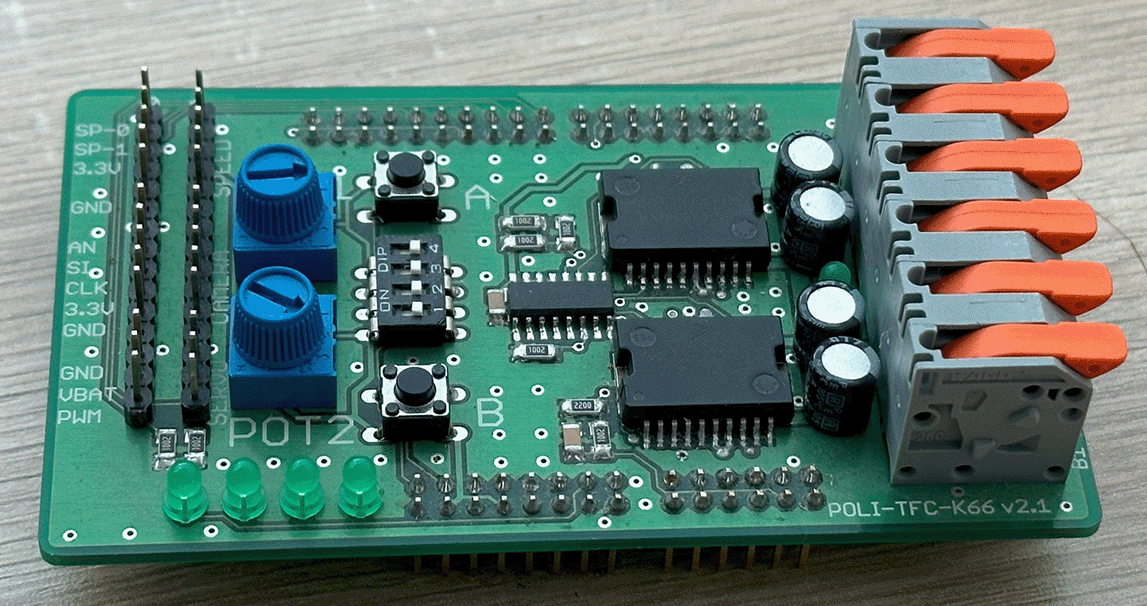
\includegraphics[width=\textwidth, height = 5cm]{Figures/POLI-TFC.png}
    	\caption{POLI-TFC.}
    	\label{fig:POLI-TFC}
	\end{subfigure}
    \caption{Vývojová platforma FRDM-K66F a~POLI-TFC shield.}
\end{figure}

\endinput

\printbibliography[title={Seznam použité literatury}]
\addcontentsline{toc}{chapter}{Seznam použité literatury}
\end{document}
